\begin{enumerate}[label=\thesubsection.\arabic*.,ref=\thesubsection.\theenumi]

\numberwithin{equation}{enumi}
\numberwithin{figure}{enumi}


\item 
8-PSK 
Consider
\begin{align}
\textbf{y = s + n}
\end{align}

where \textbf{ s$\in$ \{$s_0$, $s_1$, $s_2$, $s_3$,$s_4$,$s_5$,$s_6$,$s_7$\}}

\begin{align}
    s_0 = 
    \begin{pmatrix}
     \sqrt{E_s} \\
     0
    \end{pmatrix}
\end{align}

\begin{align}
    s_1 = 
    \begin{pmatrix}
     \sqrt{\frac{E_s}{2}}\\
     \sqrt{\frac{E_s}{2}}
    \end{pmatrix}
\end{align}
\begin{align}
    s_2 = 
    \begin{pmatrix}
      0 \\
     \sqrt{E_s}
    \end{pmatrix}
\end{align}
\begin{align}
    s_3 = 
    \begin{pmatrix}
     -\sqrt{\frac{E_s}{2}}\\
     \sqrt{\frac{E_s}{2}}
    \end{pmatrix}
\end{align}
\begin{align}
    s_4 = 
    \begin{pmatrix}
     -\sqrt{E_s} \\
     0
    \end{pmatrix}
\end{align}
\begin{align}
    s_5 = 
    \begin{pmatrix}
     -\sqrt{\frac{E_s}{2}}\\
     -\sqrt{\frac{E_s}{2}}
    \end{pmatrix}
\end{align}
\begin{align}
    s_6 = 
    \begin{pmatrix}
     0\\
     -\sqrt{E_s}
    \end{pmatrix}
\end{align}
\begin{align}
    s_7 = 
    \begin{pmatrix}
     \sqrt{\frac{E_s}{2}}\\
     -\sqrt{\frac{E_s}{2}}
    \end{pmatrix}
\end{align}

\begin{figure}[!ht]
                \resizebox{\columnwidth}{!}{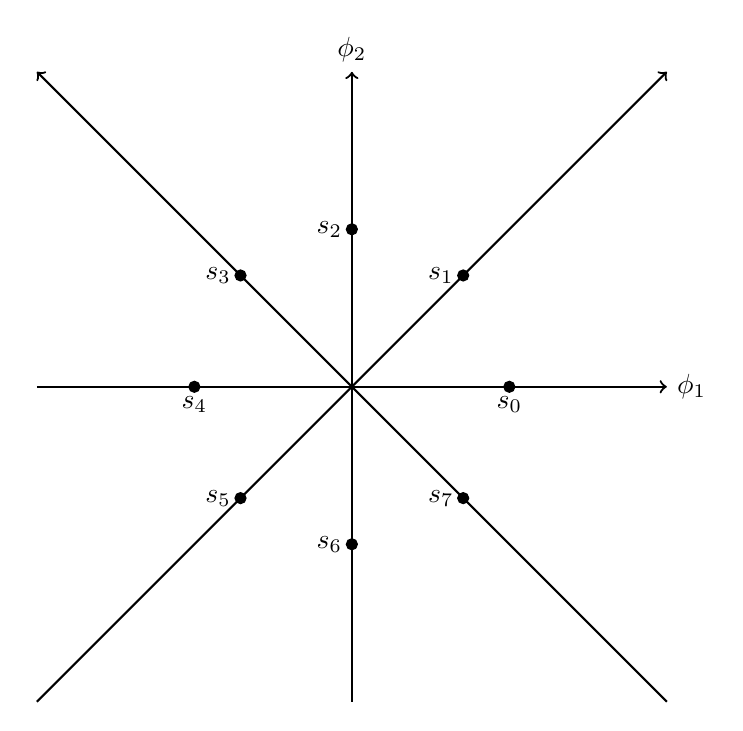
\begin{tikzpicture}

\draw[->,thick] (-4,0)--(4,0) node[right]{$\phi_1$};
\draw[->,thick] (0,-4)--(0,4) node[above]{$\phi_2$};
\draw[->,thick] (-4,-4)--(4,4) node[right]{};
\draw[->,thick] (4,-4)--(-4,4) node[above]{};

\filldraw[black] (2,0) circle (2pt) node[below] {$s_0$} ;
\filldraw[black] (1.414,1.414) circle (2pt) node[left] {$s_1$} ;
\filldraw[black] (0,2) circle (2pt) node[left] {$s_2$} ;
\filldraw[black] (-1.414,1.414) circle (2pt) node[left] {$s_3$} ;
\filldraw[black] (-2,0) circle (2pt) node[below] {$s_4$} ;
\filldraw[black] (-1.414,-1.414) circle (2pt) node[left] {$s_5$} ;
\filldraw[black] (0,-2) circle (2pt) node[left] {$s_6$} ;
\filldraw[black] (1.414,-1.414) circle (2pt) node[left] {$s_7$} ;


\end{tikzpicture}
}
\label{fig:ee18btech11012_fig1}
\caption{Constellation diagram}
\end{figure}


\item Encoding

$s_0$ denote bits 000, $s_1$ denote bits 001, $s_2$ denote bits 011,$s_3$ denote bits 010,$s_4$ denote bits 110,$s_5$ denote bits 111,$s_6$ denote bits 101,$s_7$ denote bits 100.

\item Decoding



\begin{figure}[!ht]

                \resizebox{\columnwidth}{!}{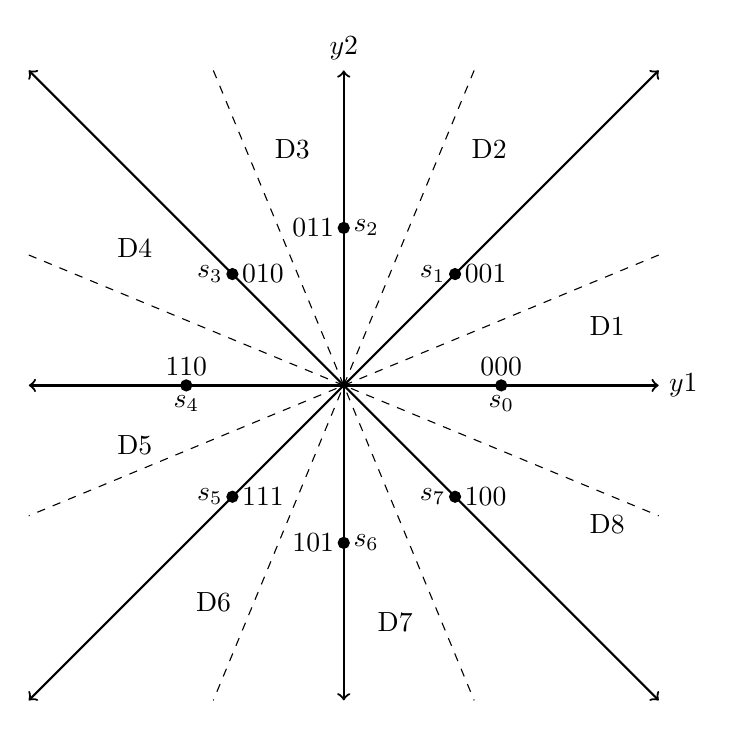
\begin{tikzpicture}

\draw[<->,thick] (-4,0)--(4,0) node[right]{$y1$};
\draw[<->,thick] (0,-4)--(0,4) node[above]{$y2$};
\draw[dashed] (4,1.656)--(-4,-1.656);
\draw[dashed] (1.656,4)--(-1.656,-4);
\draw[dashed] (-1.656,4)--(1.656,-4);
\draw[dashed] (-4,1.656)--(4,-1.656);
\draw[<->,thick](-4,-4)--(4,4);
\draw[<->,thick](-4,4)--(4,-4);

\filldraw[black] (2,0) circle (2pt) node[below] {$s_0$} node[above] {000};
\filldraw[black] (1.414,1.414) circle (2pt) node[left] {$s_1$} node[right] {001};
\filldraw[black] (0,2) circle (2pt) node[right] {$s_2$} node[left] {011};
\filldraw[black] (-1.414,1.414) circle (2pt) node[left] {$s_3$} node [right] {010};
\filldraw[black] (-2,0) circle (2pt) node[below] {$s_4$} node[above] {110};
\filldraw[black] (-1.414,-1.414) circle (2pt) node[left] {$s_5$} node[right] {111};
\filldraw[black] (0,-2) circle (2pt) node[right] {$s_6$} node[left] {101};
\filldraw[black] (1.414,-1.414) circle (2pt) node[left] {$s_7$} node [right] {100};

\foreach \coordinate/\label/\pos in {{(3,1)/D1/below right},{(1.5,3)/D2/right},{(-1,3)/D3/right},{(-3,1.5)/D4/above right},{(-3,-1)/D5/above right},{(-2,-3)/D6/above right},{(1,-3)/D7/left},{(3,-2)/D8/above right}} \node[\pos] at \coordinate {\label};

\end{tikzpicture}
}

\label{fig:ee18btech11012_fig2}
\caption{decision regions}
	
\end{figure}





Let \textbf{r} be the received bits, \textbf{r} = [$r_1$,$r_2$,$r_3$]. 
\begin{align}
    r_1 = 
    \begin{cases}
    0, &  \textbf{y} \in D1\cup D2\cup D3\cup D4 \Leftrightarrow  $y_1($\sqrt{2}-1$)+y_2>0$\\
    1, &  \textbf{y} \in D5\cup D6\cup D7\cup D8 \Leftrightarrow $y_1($\sqrt{2}-1$)+y_2<0$
    \end{cases}
    \label{eq:ee18btech11012_eq1}
\end{align}
\begin{align}
    r_2 = 
    \begin{cases}
    0, &  \textbf{y} \in D2\cup D1\cup D8\cup D7 \Longleftrightarrow $ y_2 -(\sqrt{2}+1)y_1<0$\\
    1, &  \textbf{y} \in D3\cup D4\cup D5\cup D6 \Longleftrightarrow  $y_2 -(\sqrt{2}+1) y_1 > 0$
    \end{cases}
    \label{eq:ee18btech11012_eq2}
\end{align}
\begin{align}
    r_3 = 
    \begin{cases}
    0, &  \textbf{y} \in D4\cup D5\cup D1\cup D8 \Longleftrightarrow  $y_2 +(\sqrt{2}+1)y_1 < 0$ ,  $y_2 -(\sqrt{2}-1)y_1 > 0$  \\
    1, &  \textbf{y} \in D2\cup D3\cup D6\cup D7 \Longleftrightarrow $ y_2 +(\sqrt{2}+1)y_1 > 0$ ,  $y_2 -($\sqrt{2}-1$)y_1 < 0$ 
    \end{cases}
    \label{eq:ee18btech11012_eq3}
\end{align}

From eq.\ref{eq:ee18btech11012_eq1},eq.\ref{eq:ee18btech11012_eq2} and eq.\ref{eq:ee18btech11012_eq3}
\\
For detecting $s_0$, $y_2+(\sqrt{2}-1)y_1>0$ and $y_2-(\sqrt{2}-1)y_1<0$.
\\
For detecting $s_1$, $y_2-(\sqrt{2}+1)y_1<0$ and $y_2-(\sqrt{2}-1)y_1>0$.
\\
For detecting $s_2$, $y_2-(\sqrt{2}+1)y_1>0$ and $y_2+(\sqrt{2}+1)y_1>0$.
\\
For detecting $s_3$, $y_2+(\sqrt{2}-1)y_1>0$ and $y_2+(\sqrt{2}+1)y_1<0$.
\\
For detecting $s_4$, $y_2+(\sqrt{2}-1)y_1<0$ and $y_2-(\sqrt{2}-1)y_1>0$.
\\
For detecting $s_5$, $y_2-(\sqrt{2}+1)y_1>0$ and $y_2-(\sqrt{2}-1)y_1<0$.
\\
For detecting $s_6$, $y_2-(\sqrt{2}+1)y_1<0$ and $y_2+(\sqrt{2}+1)y_1<0$.
\\
For detecting $s_7$, $y_2+(\sqrt{2}-1)y_1<0$ and $y_2+(\sqrt{2}+1)y_1>0$.




\item The following code has simulation of 8PSK.
\begin{lstlisting}
 codes/8psk.py
\end{lstlisting}




















\end{enumerate}
